

\chapter{Option pricing with transaction costs}\label{Chapter5}
%\blindtext
\minitoc% Creating an actual minitoc

\vspace{5em}

\section{Portfolio selection problems}
In the mathematical finance literature, the first application of stochastic optimal control theory to finance appears in the seminal paper \cite{Me69}.
This is the classical \emph{Merton optimal portfolio problem}, and is formulated as follows. An investor has a portfolio consisting of two assets, one ``risk free" asset $B$,
and one ``risky" asset $S$. The assets in the portfolio have dynamics
\begin{equation}\label{Merton_problem1}
 \begin{cases}
 dB_t &=  rB_t dt \\
 dS_t &=  S_t \left( \mu dt + \sigma dW_t \right),
\end{cases}
\end{equation} 
with $\mu>r$ and $\sigma>0$. We denote by $\mathcal{W}_t = \omega^1_t B_t + \omega^2_t S_t$  the wealth at time $t$, where $\omega^1_t, \omega^2_t \in \R$ 
are the quantities of the two assets held at time $t$.
It is common to introduce the fraction $\pi_t$ of wealth invested in the risky asset. 
In this way, it is possible to write
$\omega^2_t S_t = \pi_t \mathcal{W}_t$ and $\omega^1_t B_t = (1-\pi_t) \mathcal{W}_t$ and the wealth equation becomes simply 
$\mathcal{W}_t = \pi_t \mathcal{W}_t + (1-\pi_t) \mathcal{W}_t$. \\ 
The model also considers the investor consumption $\{c_t\}_{0 \leq t \leq T}$. 
The optimization problem can be formulated considering the utility function of the consumption and the terminal condition. It consists in maximizing the objective function
\begin{equation}
 J(x;\pi,c) = \E_x \biggl[ \int_0^{T} e^{-\beta t} \mathcal{U}(c_t) dt + g(T,\mathcal{W}_T) \biggr],
\end{equation}
where $\beta > 0$ and $\mathcal{U}: [0,\infty) \to \R$ is a concave and increasing utility function, such that $\mathcal{U}(0)=0$.
In the original article, the function $g$ is called \emph{bequest valuation function} and is assumed to be concave.
We indicate the initial portfolio state with $x = (B_0,S_0)$. 
The wealth $\mathcal{W}$ takes value in $\OO = (0,\infty)$ and has state dynamics
\begin{equation}
 d \mathcal{W}_t = (1-\pi_t) \mathcal{W}_t r dt + \pi_t \mathcal{W}_t (\mu dt + \sigma dW_t) - c(t)dt.
\end{equation}
The control $\alpha_t$ is a two dimensional vector $(\alpha^1_t,\alpha^2_t) = (\pi_t,c_t)$, with values in $A = \R \times [0,\infty)$. 
This is a finite horizon problem with an objective function of type (\ref{cost_functional})
and HJB equation as in (\ref{DPE}). 
Even if in this case the control space $A$ is not compact, the supremum in (\ref{DPE}) is attained, thanks to the concave structure of the problem.

Merton, using the utility $\mathcal{U}(c) = \frac{1}{\gamma} c^{\gamma}$ with $0<\gamma<1$ (of HARA type) obtained an explicit solution for the problem. In particular he found that 
the optimal control
\begin{equation}\label{Merton_policy}
  \pi^*_t = \frac{\mu-r}{(1-\gamma)\sigma^2}
\end{equation}
is a constant and does not depend on the state variables.  
This means that the optimal fraction of the risky and risk free assets in the portfolio is constant.
The line containing all the optimal points in the $(B,S)$-plane is the so called \textbf{Merton line}.

%In Chapter \ref{Chapter4} we have not considered infinite horizon control problems because they are not relevant for the thesis.
%The Merton optimal portfolio problem can be formulated as well in a finite time horizon setting, and removing the consumption rate. The objective function becomes
%\begin{equation}\label{Merton_problem2}
% J(t,x;\pi) = \E_{t,x} \biggl[ \mathcal{U}\biggl( \mathcal{W}^{\pi}(T) \biggr) \biggr] \quad \mbox{ for } \quad t \in [t_0,T].
%\end{equation}
%It turns out that the finite horizon solution is the same as the original infinite horizon Merton problem. The optimal policy is still given by formula (\ref{Merton_policy}).
%For the explicit derivation see for instance \cite{Pham}.

\noindent
The Merton portfolio selection problem is the first optimal portfolio problem solved by stochastic control theory methods. 
In \cite{Me71} the author extends the results to different utility functions.
All the successive models are generalizations of the Merton model, where by 
the word ``generalizations", we mean that under some particular choices of the parameters, the Merton problem is included in those models as a special case.
For what concerns this thesis, we review the main portfolio selection problems that have appeared in the literature, considering the presence of proportional transaction costs.
The first portfolio selection model with transaction costs and consumption was introduced by \cite{Co86} and then extended by \cite{DaNo90}. We refer to \cite{ShSo94}
for a viscosity solution approach to the same problem. 
Other important contributions are 
\cite{DaYi09}, \cite{Dai10}, \cite{LiuLo02}, \cite{LiuLo07}, \cite{BKR01}, \cite{OkSu01}, \cite{Kab16} where the last four articles use Lévy processes to model the stock dynamics. 
All the cited works are portfolio optimization models formulated as infinite horizon problems, and do not involve the pricing of the options.

Further assumptions are needed when the portfolio process is introduced for the purpose of pricing a derivative contract.
The main contributions on option pricing with transaction costs, using the \emph{indifference pricing} approach are
\cite{HoNe89} and \cite{DaPaZa93}. The problem is formalized as a finite horizon singular stochastic control problem.
In this section we present the Davis-Panas-Zariphopoulou (DPZ) model, 
which is the building block of this thesis, and then extend it following the framework introduced by \cite{Kab16}, 
that consider the stock dynamics described by Lévy processes.



\subsection{Davis-Panas-Zariphopoulou model}\label{DPZ_sec}

This is the market model with proportional transaction costs presented in \cite{DaPaZa93}. 
The authors consider a portfolio composed by one risk-free asset $B$ (bank account) paying a fixed interest rate $r > 0$ and a stock $S$. 
The symbol $Y$ denotes the number of shares of the stock $S$ that the investor holds. 
The state of the portfolio at time $t\in [t_0,T]$ is $(B^{\pi}_t,Y^{\pi}_t,S_t)$, and is the solution of the following SDE:
\begin{equation}\label{DPZ_porfolio_dynamics}
 \begin{cases}
 dB^{\pi}_t &=  rB^{\pi}_t dt - (1+\theta_b)S_t dL_t + (1-\theta_s) S_t dM_t \\
 dY^{\pi}_t &=  dL_t - dM_t \\
 dS_t &=  S_t \left( \mu dt + \sigma dW_t \right).
\end{cases}
\end{equation} 
%for a particular strategy $\{\pi_t\}_{t \in [t_0,T]} := \{(L_t,M_t)\}_{t \in [t_0,T]}$.
for $\mu>r$ and $\sigma>0$.
The parameters $\theta_b$, $\theta_s \geq 0$ are the proportional transaction costs when buying and selling respectively.
This portfolio equation is a generalization of the portfolio in the Merton problem (\ref{Merton_problem1}), 
where a new state variable $Y$ is considered.
The control process $\{\pi_t\}_{t \in [t_0,T]} := \{(L_t,M_t)\}_{t \in [t_0,T]}$ represents the trading strategy and indicates the 
cumulative number of shares bought and sold respectively in $[t_0,T]$.
The strategy $\pi_t$ is a cádlág, $\mathcal{F}^W_t$-progressively measurable, nondecreasing process with bounded variation in every finite time interval and such that
$ \pi_{t_0^-} = ( L_{t_0^-} , M_{t_0^-} ) = (0,0) $, allowing for an initial transaction at $t_0$.\\
In the discontinuity points of $L_t$ and $M_t$ we indicate the process variation with $\Delta L_t= L_{t}-L_{t^-}$ and $\Delta M_t= M_{t}-M_{t^-}$.

% In order to understand better the mechanism, let us make a recap:
% \begin{itemize}
%  \item Variation in the number of shares:
%  $$\Delta Y^{\pi}_t =  \underbrace{\Delta L_t}_{\mbox{shares bought}} - \underbrace{\Delta M_t}_{\mbox{shares sold}} $$
%  \item Variation in the bank account:
%  $$ \Delta B^{\pi}_t =  - \underbrace{(1+\theta_b)S_t}_{\mbox{adjusted price}} \Delta L_t + \underbrace{(1-\theta_s) S_t}_{\mbox{adjusted price}} \Delta M_t $$
% \end{itemize}
% we can identify this problem as a singular stochastic control problem as described in Chapter \ref{singular_control}.


\begin{Definition}
We define the \textbf{cash value} function $c(y,s)$ as the value in cash when the shares in the portfolio are liquidated, i.e.  
long positions are sold and short positions are covered.
\begin{equation}\label{cost_function}
c(y,s) = \begin{cases} 
(1+\theta_b)ys, & \mbox{if } y\leq 0 \\ 
(1-\theta_s)ys, & \mbox{if } y>0 . 
\end{cases} 
\end{equation} 
\end{Definition}
\begin{Definition}
For $t\in [t_0,T]$, we define the \textbf{total wealth} process:
\begin{equation}\label{wealth_process}
 \mathcal{W}^{\pi}_t = B^{\pi}_t + c(Y^{\pi}_t,S_t).
\end{equation} 
\end{Definition}
We say that a portfolio is solvent if the portfolio's wealth $\mathcal{W}_t$ is greater than a fixed constant $-C$, with 
$C\geq0$ that may depend on the initial wealth and on the parameters in (\ref{DPZ_porfolio_dynamics}). 
This constant may be interpreted as the \emph{credit availability} of the investor.
\begin{Definition}
We define the \textbf{solvency region}:
\begin{equation}\label{solvency_region}
 \mathcal{S} := \biggl\{ (b,y,s) \in \R \times \R \times \R^+ : b + c(y,s) > -C  \biggr\}.
\end{equation} 
\end{Definition}
\begin{Definition}\label{admissible_strategies1}
The set of \textbf{admissible trading strategies} $\Pi(t_0,b,y,s)$, is defined   
as the set of all right-continuous, nondecreasing, $\mathcal{F}_t$-progressively measurable processes  
$\{\pi_t\}_{t \in [t_0,T]}$, such that $(B^\pi_t,Y^\pi_t,S_t)$ is a solution of (\ref{DPZ_porfolio_dynamics}) with initial values $(B^\pi_{t_0} = b, Y^\pi_{t_0} = y, S_{t_0} = s)$, 
and 
\begin{equation}
 (B^\pi_t,Y^\pi_t,S_t) \in \mathcal{S}
\end{equation}
for $t \in [t_0,T]$ almost surely.
\end{Definition}

% \begin{Remark}
% In the first problem formulation of \cite{HoNe89}, the authors 
% consider a portfolio starting with zero total wealth. 
% The writer (or buyer) of the option creates a portfolio at time $t_0$ with the purpose of hedging the option.
% It is reasonable to assume that no shares of the underlying stock are contained in the portfolio at time $t_0$. 
% In the numerical computations of Chapter \ref{Chapter6}, we will consider portfolios with zero initial shares and initial cash amount $B_0$. 
% The model is able to compute option prices for an investor with any initial number $Y_0$ of shares if needed.
% \end{Remark}



\subsubsection{Utility maximization}


Let us assume an investor builds a portfolio with cash, shares of a stock and in addition he sells or purchases a 
European call option written on the same stock, with strike price $K$ and expiration date $T$.\\
From now on, we introduce the superscripts $w$, $b$ and $0$ to indicate the writer, buyer and zero-option portfolios respectively.
In the zero-option portfolio, the wealth process $\{\mathcal{W}^{0; \pi}_t\}_{t \in [t_0,T]}$ corresponds to (\ref{wealth_process}).
\begin{Definition}
For $t \in [t_0,T]$, we define the wealth processes for the writer:
  \begin{align}\label{wealth_writer}
   \mathcal{W}^{w; \pi}_t := & \; B^{\pi}_t + c(Y^{\pi}_t,S_t) \mathbbm{1}_{\{t < T\}} \\ \nonumber
   & + c(Y^{\pi}_t,S_t) \mathbbm{1}_{\{t = T,\, S_t(1+ \theta_b ) \leq K\}}
   + \biggl( c\bigl( Y^{\pi}_t-1,S_t \bigr) + K \biggr) \mathbbm{1}_{\{t=T,\, S_t(1+ \theta_b ) > K \}}
  \end{align}
 and the buyer:
  \begin{align}\label{wealth_buyer}
   \mathcal{W}^{b; \pi}_t := & \; B^{\pi}_t + c(Y^{\pi}_t,S_t) \mathbbm{1}_{\{t < T\}} \\ \nonumber
   & + c(Y^{\pi}_t,S_t) \mathbbm{1}_{\{t = T,\, S_t(1+ \theta_b ) \leq K\}}
   + \biggl( c\bigl( Y^{\pi}_t+1,S_t \bigr) - K \biggr) \mathbbm{1}_{\{t=T,\, S_t(1+ \theta_b ) > K \}}.
  \end{align}
\end{Definition}

\begin{figure}[t!]
 \centering
 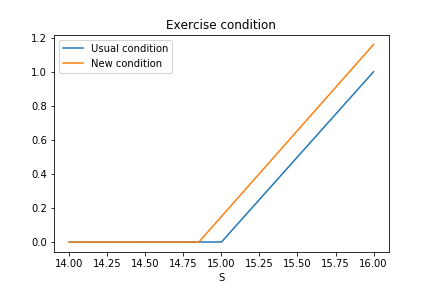
\includegraphics[scale=0.5]{payoff_comparison.png}
 % payoff_comparison.png: 0x0 pixel, 300dpi, 0.00x0.00 cm, bb=
 \caption{Comparison of exercise conditions for a European Call option with strike $K=15$, in a market with zero costs and in a market with $\theta_b=0.01$.}
 \label{fig:payoff_comparison}
\end{figure}
In the case the option is exercised, $S_T(1+ \theta_b ) > K$, the buyer pays to the writer the strike value $K$ in cash, 
and the writer delivers one share to the buyer.
In a market with transaction costs the real value (in cash) of a share incorporates the transaction costs. 
Therefore the buyer does not exercise when $S_T > K$, but when $S_T(1+ \theta_b ) > K$. 
In Figure \ref{fig:payoff_comparison} there is a comparison between the exercise conditions in a market with zero costs (as in Black-Scholes) and in a market with 
transaction costs.

The objective of the investor is to maximize the expected utility of the wealth at terminal time $T$ over all the admissible
strategies. This expectation is conditioned on the current value of cash, number of shares and value of the
stock.
The sets of trading strategies corresponding to each of the three portfolios, is obtained by using the respective wealth process inside Definition [\ref{admissible_strategies1}]. 

\begin{Definition}
 The \textbf{value function} of the maximization problem for $j=w,b,0$ is defined as:
\begin{align}\label{max_probl0}
V^j(t,b,y,s) := \sup_{\pi \in \Pi^j(t,b,y,s)} \; & \E_{t,b,y,s}\biggl[ 
            \mathcal{U}(\mathcal{W}^{j; \pi}_T) \biggr],             
\end{align}
where $\mathcal{U}: \R \to \R$ is a concave increasing utility function such that $\mathcal{U}(0)=0$.
\end{Definition}
Let us verify that the cost function is well defined. Let us consider only the case $j=0$, because for $j=w,b$ the generalization is straightforward.
\begin{Theorem}
The objective function is finite, i.e.
$$ \E_{t,b,y,s}\biggl[ \mathcal{U}(\mathcal{W}^{\pi}_T) \biggr] < \infty$$
for all $\pi \in \Pi(t,b,y,s)$.
\end{Theorem}
\begin{proof}
 Since the utility function is concave, thanks to the Jensen inequality $\E_{t,b,y,s} \bigl[\mathcal{U}(\mathcal{W}^{\pi}_T)\bigr] \leq 
 \mathcal{U}\bigl( \E_{t,b,y,s}[\mathcal{W}^{\pi}_T] \bigr)$,
 it is enough to prove $\E_{t,b,y,s}[\mathcal{W}^{\pi}_T] < \infty$.\\
 The wealth at time $T$ is:
 \begin{align*}
   \mathcal{W}^{\pi}_T &=  B^{\pi}_T + c(Y^{\pi}_T,S_T) \\
                       &\leq B^{\pi}_T + Y^{\pi}_T S_T.
 \end{align*}
 where $B^{\pi}_T$ is the solution of the first line of (\ref{DPZ_porfolio_dynamics}) i.e.
 \begin{equation*}
 B^{\pi}_T =  \frac{b}{\delta(t,T)} - \int_{t}^T
 (1+\theta_b)\frac{S_u}{\delta(u,T)} dL_u + \int_{t}^T
 (1-\theta_s) \frac{S_u}{\delta(u,T)} dM_u 
 \end{equation*}
 with $\delta(u,T) = e^{-r(T-u)}$.  
 By taking the expectation we get
 \begin{align*}
 \E_{t,b,y,s}\biggl[ \int_{t}^T (1+\theta_b)\frac{S_u}{\delta(u,T)} dL_u  \biggr] & \leq \frac{(1+\theta_b)}{\delta(t,T)} 
                                                                                    \E_{t,b,y,s}\biggl[ \biggl(\max_{u\in[t,T]} S_u \biggr)\int_{t}^T dL_u  \biggr] \\
                                                                                &\leq \frac{(1+\theta_b)}{\delta(t,T)} \E_{t,b,y,s}\biggl[ \biggl(\max_{u\in[t,T]} S_u \biggr) L_T  \biggr] 
 \end{align*}
where for simplicity we assume $L_t=0$.
Let us define the running maximum $\mathcal{M}_T := \max_{u\in[t,T]} S_{u}$. 
The term $\E \bigl[ (\mathcal{M}_T)^2 \bigr] < \infty$ because of (\ref{cond_3}).
We also know that $\E \bigl[ (L_T)^2 \bigr] < \infty $ because of the assumption (\ref{singular_moments}).
Now we can use the Schwartz inequality and obtain:
\begin{equation}
  \E_{t,b,y,s} \bigl[ \mathcal{M}_T L_T \bigr]^2  \leq \E_{t,b,y,s}[(\mathcal{M}_T)^2] \, \E_{t,b,y,s} \bigl[ (L_T)^2 \bigr] < \infty.
\end{equation}
The same argument can be applied to $\E_{t,b,y,s}\bigl[ \int_{t}^T (1-\theta_s) \frac{S_u}{\delta(u,T)} dM_u \bigr]$.\\
By using again the Schwartz inequality, we can verify that $\E_{t,b,y,s}\bigl[ Y^{\pi}_T S_T \bigr] = \E_{t,b,y,s}\bigl[ S_T(L_T - M_T) \bigr]$ is finite as well.
And this concludes the proof.
\end{proof}



The writer (buyer) option price is defined as the amount of cash to add (subtract) to the bank account, 
such that the maximal expected utility of wealth of the writer (buyer) is the same he could get with 
the zero-option portfolio.
\begin{Definition}
The writer price is the value $p^w>0$ such that 
 \begin{equation}\label{writer}
  V^0(t,b,y,s) = V^w(t,b+p^w,y,s),
 \end{equation}
 and the buyer price is the value $p^b>0$ such that
 \begin{equation}\label{buyer}
  V^0(t,b,y,s) = V^b(t,b-p^b,y,s).
 \end{equation}
\end{Definition}


\subsubsection{HJB Equation}\label{subsec_HJB}

According to the theory of stochastic optimal control presented in Chapter \ref{Chapter4},  
we can identify the DPZ model within the class of singular control problems described in Section (\ref{singular_control}).
Let us re-write the state equation (\ref{DPZ_porfolio_dynamics}) for $X^{\pi}_t = (B^{\pi}_t,Y^{\pi}_t,S_t)$ in matrix form 
\begin{align}\label{DPZ_porfolio_dynamicsM}
d X^{\pi}_t
=& 
 d \left(
\begin{array}{l}
B^{\pi}_t\\
Y^{\pi}_t\\
S_t
\end{array} \right) \\ \nonumber
  =&  \left( \begin{array}{l}
r B^{\pi}_t\\
0\\
\mu S_{t}
\end{array} \right)
dt +  \left( \begin{array}{l}
0\\
0\\
\sigma S_{t}
\end{array} \right) dW_t \\ \nonumber
&+ \underbrace{\left( \begin{array}{cc}
-S_{t}(1+\theta_b) & S_{t}(1-\theta_s) \\
1 & -1 \\
0 & 0
\end{array} \right)}_{\kappa(t,X_t)}
\underbrace{\left( \begin{array}{l}
dL_t \\
dM_t 
\end{array} \right)}_{d\xi_t},
\end{align}
which can be easily identified with the general equation (\ref{singular_SDE}).
The state $X^{\pi}_t$ takes values in $\OO$ corresponding to the solvency region $\SI$.
The objective function that we maximize in Eq. (\ref{max_probl0}) corresponds to Eq. (\ref{singular_cost_functional}) with $\hat f$ and $h$ equal to zero. 

Let us check that the Frobenius condition (\ref{Frobenius}) is satisfied.
Let us call $\tilde \theta_b = (1+\theta_b)$ and $\tilde \theta_s = (1-\theta_s)$.  The commutator is:
\begin{equation}
 \left( \begin{array}{ccc}
0 & 0 & -\tilde \theta_b \\
0 & 0 & 0 \\
0 & 0 & 0
\end{array} \right)
\left( \begin{array}{l}
 S_{t}\tilde \theta_s \\
-1 \\
0
\end{array} \right) -
 \left( \begin{array}{ccc}
0 & 0 & \tilde \theta_s \\
0 & 0 & 0 \\
0 & 0 & 0
\end{array} \right)
\left( \begin{array}{l}
-S_{t}\tilde \theta_b \\
1 \\
0
\end{array} \right) = 0
\end{equation}
which shows that the condition is satisfied.

According to singular control theory, the HJB equation of a singular control problem is a variational inequality. Here we can obtain the HJB equation of this problem 
from the general equation (\ref{variational_inequality}). We omit the subscript of $V^j$ when the discussion refers to all the three problems. 
Let us indicate $x = (b,y,s)$. Let us consider:
$$ D_x V(t,x) = \left( \frac{\partial V(t,b,y,s)}{\partial b}, \frac{\partial V(t,b,y,s)}{\partial y}, \frac{\partial V(t,b,y,s)}{\partial s} \right) $$
and
$$ \hat K := \biggl \{ \biggl( \begin{array}{c} l \\ m \end{array} \biggr) \in [0,\infty) \times [0,\infty): |l|^2 + |m|^2 = 1 \biggr \}. $$ 
Following (\ref{set_K}) we obtain
\begin{align*}
& \sup_{l,m \in \hat K}
\left( \frac{\partial V}{\partial b}, \frac{\partial V}{\partial y}, \frac{\partial V}{\partial s} \right)
\left( \begin{array}{cc}
-s(1+\theta_b) & s(1-\theta_s) \\
1 & -1 \\
0 & 0
\end{array} \right)
\left( \begin{array}{c}
l \\
m 
\end{array} \right) \\ 
= & \sup_{l,m \in \hat K}
\frac{\partial V}{\partial b} \biggl( -s(1+\theta_b)l + s(1-\theta_s)m \biggr) +
\frac{\partial V}{\partial y} \bigl( l-m \bigr) \\
= & \sup_{l,m \in \hat K}
l \biggl( -s(1+\theta_b)\frac{\partial V}{\partial b} + \frac{\partial V}{\partial y} \biggr) +
m \biggl( s(1-\theta_s)\frac{\partial V}{\partial b} - \frac{\partial V}{\partial y} \biggr)
\end{align*}

\vspace{3em}
\noindent
The terms 
$$ \biggl( -s(1+\theta_b)\frac{\partial V}{\partial b} + \frac{\partial V}{\partial y} \biggr) 
\quad \mbox{and} \quad \biggl( s(1-\theta_s)\frac{\partial V}{\partial b} - \frac{\partial V}{\partial y} \biggr)  $$
cannot be positive at the same time, otherwise we would get
$$ s(1+\theta_b)\frac{\partial V}{\partial b} < \frac{\partial V}{\partial y} < s(1-\theta_s)\frac{\partial V}{\partial b} $$
which is impossible for $s,\theta_b,\theta_s>0$. \\

\noindent
The other possibilities are 
\begin{enumerate}
 \item $\biggl(-s(1+\theta_b)\frac{\partial V}{\partial b} + \frac{\partial V}{\partial y}\biggr) > 0$ 
 and $\biggl(s(1-\theta_s)\frac{\partial V}{\partial b} - \frac{\partial V}{\partial y}\biggr) \leq 0$. \\ The optimal control is $l=1$ and $m=0$.
 \item $\biggl(-s(1+\theta_b)\frac{\partial V}{\partial b} + \frac{\partial V}{\partial y}\biggr) \leq 0$
 and $\biggl(s(1-\theta_s)\frac{\partial V}{\partial b} - \frac{\partial V}{\partial y}\biggr) > 0$. \\ The optimal control is $l=0$ and $m=1$.
 \item $\biggl(-s(1+\theta_b)\frac{\partial V}{\partial b} + \frac{\partial V}{\partial y}\biggr) < 0$ and 
 $\biggl(s(1-\theta_s)\frac{\partial V}{\partial b} - \frac{\partial V}{\partial y}\biggr) < 0$. \\ The optimal control is $l=0$ and $m=1$ or $l=1$ and $m=0$, depending on which term 
 is bigger.
\end{enumerate}

\noindent
We should also consider the case when both are zero, which happens for 
$$\frac{\partial V}{\partial b} = \frac{\partial V}{\partial y} = 0.$$ 
But this is not possible because the function $V$ is an increasing function of $b$ and $y$ 
(for a proof see Theorem 5.3.4 in \cite{Damgaard}).
Intuitively, this can be explained by thinking that an extra initial wealth provides higher final expected utility.

\noindent
From this argument we derived the optimal set $\hat K = \left( \begin{array}{c}
			   1 \\
			   0
                          \end{array} \right) \bigcup \left( \begin{array}{c}
			   0 \\
			   1
                          \end{array} \right)$.

Considering again Eq. (\ref{set_K}), together with the optimal set $\hat K$,
we obtain
$$ H \bigl(t,x, D_x V(t,x) \bigr) = \max \biggl\{ \frac{\partial V}{\partial y}-(1+\theta_b) s \frac{\partial V}{\partial b} ,
 -\bigl( \frac{\partial V}{\partial y} -(1-\theta_s)s \frac{\partial V}{\partial b} \bigr) \biggr\}. $$

\noindent 
The resulting HJB equation is
\begin{align}\label{DPZ_HJB}
& \max \; \biggl\{ \; \frac{\partial V}{\partial t} + rb\frac{\partial V}{\partial b} 
+ \mu s \frac{\partial V}{\partial s} + \frac{1}{2}\sigma^2 s^2 \frac{\partial^2 V}{\partial s^2}, \\ \nonumber
& \;  \frac{\partial V}{\partial y}-(1+\theta_b) s \frac{\partial V}{\partial b} \; 
, \; -\biggl(\frac{\partial V}{\partial y}-(1-\theta_s)s \frac{\partial V}{\partial b} \biggr) \biggr\} = 0, 
\end{align}
for $(t,b,y,s) \in [t_0,T] \times \SI$.
The terminal conditions for the three portfolio problems $j=0,w,b$ are:
\begin{equation}\label{terminal_conditions}
V^j(T,b,y,s) = \mathcal{U}\bigl( w^j(b,y,s) \bigr) \hspace{1em} \mbox{ for } \hspace{1em} (b,y,s) \in \mathcal{S}^j 
\end{equation}
with
  \begin{equation*}
   w^0(b,y,s) =  b + c(y,s).
  \end{equation*}
  \begin{equation*}
   w^w(b,y,s) =  b + c(y,s) \mathbbm{1}_{\{ s(1+\theta_b) \leq K\}} +
  \biggl( c\bigl( y-1,s \bigr) + K \biggr) \mathbbm{1}_{\{s(1+\theta_b)>K\}}.
  \end{equation*}
  \begin{equation*}
   w^b(b,y,s) = b + c(y,s) \mathbbm{1}_{\{ s(1+\theta_b) \leq K\}} +
  \biggl( c\bigl( y+1,s \bigr) - K \biggr) \mathbbm{1}_{\{s(1+\theta_b)>K\}}.
  \end{equation*}

\noindent
The variational inequality (\ref{DPZ_HJB}) says that the maximum of three operators is equal to zero.
This feature can be interpreted better if we consider the state space divided into three different regions: the \textbf{Buy}, the \textbf{Sell}
and the \textbf{No Transaction} (NT) regions.
\begin{itemize}
 \item \textbf{Buy}
  \begin{equation*}
   \begin{cases}
     & \frac{\partial V}{\partial t} + rb\frac{\partial V}{\partial b} + \mu s \frac{\partial V}{\partial s} + \frac{1}{2}\sigma^2 s^2 \frac{\partial^2 V}{\partial s^2} \leq 0\\ 
     & \frac{\partial V}{\partial y}-(1+\theta_b) s \frac{\partial V}{\partial b} = 0 \\
     & -\biggl(\frac{\partial V}{\partial y}-(1-\theta_s)s \frac{\partial V}{\partial b} \biggr) \leq 0.
   \end{cases}
  \end{equation*}
 \item \textbf{Sell}
  \begin{equation*}
   \begin{cases}
     & \frac{\partial V}{\partial t} + rb\frac{\partial V}{\partial b} + \mu s \frac{\partial V}{\partial s} + \frac{1}{2}\sigma^2 s^2 \frac{\partial^2 V}{\partial s^2} \leq 0 \\ 
     & \frac{\partial V}{\partial y}-(1+\theta_b) s \frac{\partial V}{\partial b} \leq 0 \\
     & -\biggl(\frac{\partial V}{\partial y}-(1-\theta_s)s \frac{\partial V}{\partial b} \biggr) = 0.
   \end{cases}
  \end{equation*}
 \item \textbf{No Transaction}
  \begin{equation*}
   \begin{cases}
     & \frac{\partial V}{\partial t} + rb\frac{\partial V}{\partial b} + \mu s \frac{\partial V}{\partial s} + \frac{1}{2}\sigma^2 s^2 \frac{\partial^2 V}{\partial s^2} = 0 \\ 
     & \frac{\partial V}{\partial y}-(1+\theta_b) s \frac{\partial V}{\partial b} \leq 0 \\
     & -\biggl(\frac{\partial V}{\partial y}-(1-\theta_s)s \frac{\partial V}{\partial b} \biggr) \leq 0.
   \end{cases}
  \end{equation*}
\end{itemize}
The optimization problem is a free boundary problem, and its solution consists in finding the value function $V$ and the 
optimal boundaries that divide the three regions.
The Buy and Sell regions do not intersect, and are separated by the NT region. 
In the derivation of the optimal set $\hat K$, we have seen that it is not optimal to buy and sell a share at the same time. 
This is reasonable since buying and selling a share at the same time just decreases the 
total wealth, because of the transaction costs, and therefore makes no sense. 

The free boundaries of the NT region completely characterize the investor's trading strategy.
The optimal strategy consists in keeping the portfolio process inside the NT region. 
If the portfolio exits the NT region, the optimal strategy is to trade in order to bring it back to the NT region.

In the Buy and Sell regions the value functions is constant along the directions of the trades.
We get respectively:
\begin{itemize}
 \item[Buy]: \hspace{2em} $V(t,b,y,s) = V(t,b-s(1+\theta_b)\Delta L_t,y+\Delta L_t,s).$
 \item[Sell]: \hspace{2em} $ V(t,b,y,s) = V(t,b+s(1-\theta_s)\Delta M_t,y-\Delta M_t,s).$
\end{itemize}
where $\Delta L_t$ and $\Delta M_t$ are the number of shares respectively bought or sold in the trade.
%In the NT region the portfolio evolves according to the portfolio equation (\ref{DPZ_porfolio_dynamics}), with $dL=dM=0$.
%It means that the number of shares remains constant as long as the portfolio stays in the NT region.





\subsection{DPZ with jumps}\label{DPZ_j_sec}


The purpose of this thesis is to extend the DPZ model in order to include jumps in the stock dynamics. 
Following the framework of \cite{Kab16} let us introduce a market model with proportional transaction costs 
that consider an exponential Lévy process for the stock dynamics, as in \ref{exp_sde2}.
The state of the portfolio at time $t\in [t_0,T]$ is $(B^{\pi}_t,Y^{\pi}_t,S_t)$ and evolves following the SDE:
\begin{equation}\label{porfolio_dynamics}
 \begin{cases}
 dB^{\pi}_t &=  rB^{\pi}_t dt - (1+\theta_b)S_{t^-} dL_t + (1-\theta_s) S_{t^-} dM_t \\
 dY^{\pi}_t &=  dL_t - dM_t \\
 dS_t &=  S_{t^-} \left( \mu dt + \sigma dW_t + \int_{\R} (e^z-1) \tilde N(dt,dz) \right).
\end{cases}
\end{equation}
The strategy $\{\pi_t\}_{t \in [t_0,T]}$ is a cádlág, $\mathcal{F}_t$-predictable\footnote{We are considering the Wiener-Poisson filtration 
defined in Section \ref{Optimal_control_framework}.}, nondecreasing process with bounded variation, such that
$ \pi_{t_0^-} = \bigl ( L_{t_0^-} , M_{t_0^-} \bigr ) = (0,0)$. 
Under these assumptions the portfolio process 
$\bigl \{(B^{\pi}_t,Y^{\pi}_t,S_t)\bigr \}_{t \in [t_0,T]}$ has a cádlág modification, and this is what we consider.

If at time $t$ there is an unpredictable jump in the stock price $\Delta S_t = S_t - S_{t^-}$, a possible transaction should happen after the jump.
The control process $\{\pi_t\}_{t \in [t_0,T]}$ is assumed to be predictable, i.e. measurable with respect to the left-continuous filtration $\{\mathcal{F}_{t^-}\}_{t \in [t_0,T]}$.
Therefore, a jump in the price and a jump in the control cannot occur simultaneously, almost surely. 
A deeper digression on this topic can be found in Section 2 of \cite{Kab16}.   
If the investor at time $t$ observes a jump in the price and decides to rebalance his portfolio, he will trade at some time $u>t$ at the price $S_{u^-}$. 
Under this framework, as explained in \cite{Kab16}, the optimal strategy cannot exist. 

The definitions of cash value (\ref{cost_function}), of total wealth (\ref{wealth_process}), (\ref{wealth_buyer}), (\ref{wealth_writer}) and the solvency regions
(\ref{solvency_region}) are kept the same. The set of admissible trading strategy will be changed.

Since the underlying stock follows a process with jumps, it is not guaranteed that the portfolio stays
solvent for all $t \in [t_0,T]$. When holding short positions, it is possible that a sudden increase in the stock price 
causes the total wealth to jump out of the solvency region. 
The same can happen with a downward jump when the investor is long in stocks and negative in cash. 
The immediate decrease of the stock's price makes him unable to pay the debts.
\begin{Definition}
The first \textbf{exit time} from the solvency region is defined as:
\begin{equation}\label{exit_time}
 \tau := \inf \bigl\{ t \in [t_0,T] : (B^\pi_t,Y^\pi_t,S_t) \not\in \SI \bigr\}.
\end{equation} 
\end{Definition}
\begin{Definition}\label{set_trad_strat}
The set of \textbf{admissible trading strategies} $\Pi(t_0,b,y,s)$   
is the set of all cádlág, nondecreasing, predictable, bounded variation processes $\{\pi_t\}_{t \in [t_0,T]}$
such that $(B^\pi_t,Y^\pi_t,S_t)$ is a solution of (\ref{porfolio_dynamics}) with initial values $(B^\pi_{t_0} = b, Y^\pi_{t_0} = y, S_{t_0} = s)$ and such that
$\pi_t = \pi_{\tau}$ for all $t \geq \tau$.  
\end{Definition}

The objective of the investor is to maximize the expected utility of the wealth at $\tau^j \wedge T$ over all the admissible
strategies. This expectation is conditioned on the current value of cash, number of shares and value of the
stock.
\begin{Definition}
 The \textbf{value function} of the maximization problem for $j=w,b,0$ is defined as:
\begin{align}\label{max_probl1}
V^j(t,b,y,s) := \sup_{\pi \in \Pi^j(t,b,y,s)} \; & \E_{t,b,y,s}\biggl[ 
            \mathcal{U}(\mathcal{W}^{j; \pi}_T) \; \mathbbm{1}_{\{\tau^j > T\}} \\ \nonumber
             &+ e^{ \beta (T-\tau^j)} \mathcal{U}( \mathcal{W}^{j; \pi}_{\tau^j} ) \; 
             \mathbbm{1}_{\{\tau^j \leq T\}}\biggr],             
\end{align}
where $\mathcal{U}: \R \to \R$ is a concave increasing utility function such that $\mathcal{U}(0)=0$, and $\beta \geq 0$.
\end{Definition}

The HJB equation associated to this stochastic control problem is obtained following the same steps we used to derive (\ref{DPZ_HJB}). The infinitesimal generator of the price 
dynamics has the 
form (\ref{inf_gen_exp_levy}) for exponential Lévy processes. The HJB variational inequality is
\begin{align}\label{HJB1}
& \max \; \biggl\{ \; \frac{\partial V^j}{\partial t} + rb\frac{\partial V^j}{\partial b} 
+ \mu s \frac{\partial V^j}{\partial s} + \frac{1}{2}\sigma^2 s^2 \frac{\partial^2 V^j}{\partial s^2} \\ \nonumber
&+ \int_\mathbb{R}
\biggl[ V^j(t,b,y,se^z) - V^j(t,b,y,s) - s(e^z-1)\frac{\partial V^j}{\partial s} \biggr] \nu(dz) \;,\\ \nonumber
& \;  \frac{\partial V^j}{\partial y}-(1+\theta_b) s \frac{\partial V^j}{\partial b} \; 
, \; -\biggl(\frac{\partial V^j}{\partial y}-(1-\theta_s)s \frac{\partial V^j}{\partial b} \biggr) \biggr\} = 0, 
 \end{align}
for $(t,b,y,s) \in [t_0,T) \times \SI^j$ and $j=0,w,b$.   
The terminal boundary conditions are given by Eq. (\ref{terminal_conditions}).
Since this HJB equation is a PIDE,
the non-local integral operator implies to 
define the lateral conditions not only on the boundary
of the solvency region, but also beyond:
\begin{equation}\label{lat_bound}
V^j(t,b,y,s) = e^{ \beta (T-t)} \mathcal{U}\bigl( b + c(y,s)\bigr) 
\end{equation}
for $t \in [t_0,T)$ , $(b,y,s) \not \in \mathcal{S}$ and for $j=0,w,b$. 


\subsection{Variable reduction}\label{variable_reduction}


In the DPZ model introduced in Section \ref{DPZ_sec}, the portfolio is solvent for every
$t \in [t_0,T]$ and it is always possible to calculate the utility 
of the wealth at the terminal time $\mathcal{U}(\mathcal{W}^{\pi}_T)$.
In the extended model of Section \ref{DPZ_j_sec} the stock process can jump, and in presence of short positions the portfolio can go bankrupt at any time before the maturity $T$. 

With the intention of simplifying the maximization problem (\ref{max_probl1}) and reducing the number of variables, 
%we restrict our attention to the subset of solvent paths. 
we restrict our attention to the case of no bankruptcy.
A possible idea is to consider a positive initial wealth, and define the restricted set of admissible strategies as the set of $\{\pi_t\}_{t \in [t_0,T]}$ such that 
$B^{\pi}_t \geq 0$ and $Y^{\pi}_t \geq 0$ for all $t\in [t_0,T]$ (see \cite{Benth02}).
However, in order to implement a hedging strategy, we are interested in portfolios containing short positions as well.
So, we can assume that the investor has a very large credit availability $C$ in the sense that
\begin{equation}\label{P_tau}
 \PP(\tau > T) \underset{C\to \infty}{\to} 1.
\end{equation}
In practical terms, we ignore the possibility of default. The solvency region becomes $\mathcal{S} = \R^2 \times \R^{+}$ and no lateral boundary conditions are imposed.

As in \cite{DaPaZa93}, for $\gamma>0$, we consider the exponential utility function
\begin{equation}\label{exp_util}
 \mathcal{U}(x) := 1- e^{-\gamma x}.
\end{equation}
Thanks to (\ref{P_tau}) and (\ref{exp_util}) we can remove $\{B^{\pi}_t\}_{t \in [t_0,T]}$ from the state dynamics.
By solving (\ref{porfolio_dynamics}) we get
\begin{equation}\label{BT}
B^{\pi}_T =  \frac{B^{\pi}_{t}}{\delta(t,T)} - \int_{t}^T
(1+\theta_b)\frac{S_u}{\delta(u,T)} dL_u + \int_{t}^T
 (1-\theta_s) \frac{S_u}{\delta(u,T)} dM_u 
\end{equation}
where $\delta(u,T) = e^{-r(T-u)}$.
Using together (\ref{P_tau}), (\ref{exp_util}) and (\ref{BT}), and the wealth processes (\ref{wealth_process}),(\ref{wealth_writer}),(\ref{wealth_buyer}), 
we obtain for $B^\pi_{t} = b$, $Y^\pi_{t} = y$, $S_{t} = s$ and $j=0,w,b$:
\begin{align}\label{var_reduct}
   V^j(t,b,y,s) = \sup_{\pi} \; \E_{t,b,y,s}\biggl[  1- e^{-\gamma \mathcal{W}^j(T) } \biggr]  % \\ \nonumber 
	     = 1- e^{-\gamma \frac{b}{\delta(t,T)}} Q^j(t,y,s),
\end{align} 
where
\begin{align}\label{minimization}
Q^j(t,y,s) = \inf_{\pi} \; \mathbb{E}_{t,y,s}\biggl[ \; &
	     e^{-\gamma \bigl[ -\int_{t}^T (1+\theta_b) \frac{S_u}{\delta(u,T)} dL_u +
	     \int_{t}^T (1-\theta_s) \frac{S_u}{\delta(u,T)} dM_u \bigr] } \, \\ \nonumber 
	     & \times H^j(Y^{\pi}_T,S_T) \bigg]  
\end{align}
is our new minimization problem.
The exponential term inside the expectation can be considered as a discount factor, and the second term 
$H^j(y,s) = Q^j(T,y,s)$ is the terminal payoff:
\begin{itemize}
 \item No option:
 \begin{equation}\label{terminal_c}
  H^0(y,s) = e^{-\gamma \, c(y,s)}.
 \end{equation}
 \item Writer:
  \begin{equation}\label{terminal_w}
  H^w(y,s) = e^{-\gamma \bigl[ c(y,s)\mathbbm{1}_{\{s(1+\theta_b) \leq K\}} + 
 \bigl( c( y-1,s) + K \bigr) \mathbbm{1}_{\{s(1+\theta_b)>K\}} \bigr] }.
 \end{equation}
 \item Buyer:
  \begin{equation}\label{terminal_b}
  H^b(y,s) = e^{-\gamma \bigl[ c(y,s)\mathbbm{1}_{\{s(1+\theta_b) \leq K\}} + 
 \bigl( c( y+1,s) - K \bigr) \mathbbm{1}_{\{s(1+\theta_b)>K\}} \bigr] }.
 \end{equation}
\end{itemize}
Using conditions (\ref{writer}), (\ref{buyer}) together with (\ref{var_reduct}), we obtain the explicit formulas for the option prices:
\begin{equation}\label{opt_w}
 p^w(t_0,y,s) = \frac{\delta(t_0,T)}{\gamma} \log \biggl( \frac{Q^w(t_0,y,s)}{Q^0(t_0,y,s)} \biggr),
\end{equation}
\begin{equation}\label{opt_b}
 p^b(t_0,y,s) = \frac{\delta(t_0,T)}{\gamma} \log \biggl( \frac{Q^0(t_0,y,s)}{Q^b(t_0,y,s)} \biggr).
\end{equation}

Since $Q^j(t,y,s)$ is independent on $b$, let us write
$ Q^j(t,y,s) := 1 - V^j(t,0,y,s)$.
It is convenient to pass to the log-variable $x = \log(s)$, such that
\begin{equation}\label{log_var}
s \frac{\partial}{\partial s} = \frac{\partial}{\partial x}, \hspace{2em} 
s^2 \frac{\partial^2}{\partial s^2} = \frac{\partial^2}{\partial x^2} - \frac{\partial}{\partial x} . 
\end{equation}
For $j=0,w,b$, the HJB Eq. (\ref{HJB1}) becomes:
\begin{align}\label{HJB2}
& \min \; \biggl\{ \; \frac{\partial Q^j}{\partial t} + (\mu-\frac{1}{2}\sigma^2) \frac{\partial Q^j}{\partial x}
+ \frac{1}{2}\sigma^2 \frac{\partial^2 Q^j}{\partial x^2} \\ \nonumber
&+ \int_\mathbb{R}
\biggl[ Q^j(t,y,x+z) - Q^j(t,y,x) - (e^z-1)\frac{\partial Q^j}{\partial x} \biggr] \nu(dz) \;,  \\ \nonumber
& \; \frac{\partial Q^j}{\partial y} +(1+\theta_b) e^x \frac{\gamma}{\delta(t,T)}Q^j \; , 
\; -\biggl( \frac{\partial Q^j}{\partial y}+(1-\theta_s)e^x \frac{\gamma}{\delta(t,T)} Q^j 
\biggr) \biggr\} = 0. 
 \end{align}
% This equation is well defined for $Q^j \in C^{1,1,2}\bigl( (t_0,T) \times \R^2\bigr) \bigcap C_2\bigl( [t_0,T] \times \R^2 \bigr) $. 








\section{Existence of viscosity solution}\label{Existence_viscosity}

The general fact that value functions of control problems can be characterized as
viscosity solutions of certain partial differential equations is a direct consequence of the dynamic
programming principle. For singular control problems, however, the classical approach of \cite{PLL83}
fails because the state process may jump due to the singular control and it needs thus not stay
in a small ball\footnote{For processes of type (\ref{singular_SDE}) it is not possible to apply the theorem (\ref{stochastic_theorem}).} 
for a small $\Delta t$.
This problem can be circumvented by relying on the
existence of the optimal control, as done in \cite{DaPaZa93}. However, in our proof we will not assume the existence of the optimal control, because 
in this framework it does not exist (as explained in Section \ref{DPZ_j_sec} it is not possible to give an immediate response at the jump time of the stock).
We will assume that the \textbf{DPP} for the singular control problem (\ref{porfolio_dynamics}), (\ref{max_probl1}) holds, and that the value function  
is continuous. We refer to Sections 4 and 9 of \cite{Kab16} for the proofs of these statements. 

In this section we prove that the value function (\ref{max_probl1}), can be interpreted 
as the viscosity solution of the HJB equation (\ref{HJB1}).
%The proof follows the approach in \cite{OkSu01}.

Let us call $\tau_{\SI}$ the first exit time from $\SI$.
Since the stock dynamics is stochastically continuous and the control process $\pi$ cannot be the cause of bankruptcy,
we can exclude an immediate jump out of the solvency region, i.e. $\PP ( \tau_{\SI} = t_0 ) =0$.

We have to interpret the HJB equation (\ref{HJB1}) with boundary conditions (\ref{lat_bound}) and (\ref{terminal_conditions}) 
as a parabolic problem of the type (\ref{parabolic_PIDE}). 
Let us use the notation $x = (b,y,s)$ to indicate a point in $\R^2\times \R^+$. In order to satisfy the parabolic conditions we reformulate the HJB as 
\begin{align}\label{HJB22}
& \min \; \biggl\{ - \biggl( \; \frac{\partial V}{\partial t} + rb\frac{\partial V}{\partial b} 
+ \mu s \frac{\partial V}{\partial s} + \frac{1}{2}\sigma^2 s^2 \frac{\partial^2 V}{\partial s^2} \\ \nonumber
&+ \int_\mathbb{R}
\biggl[ V(t,b,y,se^z) - V(t,b,y,s) - s(e^z-1)\frac{\partial V}{\partial s} \biggr] \nu(dz) \; \biggr) ,\\ \nonumber
& \; - \biggl( \frac{\partial V}{\partial y}-(1+\theta_b) s \frac{\partial V}{\partial b} \biggr) \; 
, \; + \biggl(\frac{\partial V}{\partial y}-(1-\theta_s)s \frac{\partial V}{\partial b} \biggr) \biggr\} = 0. 
\end{align}
We indicate this function with
$ F(t,x,V,D_t V,D_{x} V,D_{xx}V,\I(t,x,V)) = 0$ in the domain $(t,x) \in [t_0,T) \times \SI$.
To simplify the notation, let us introduce the integro-differential infinitesimal generator:
\begin{align*}
 \LL V(t,x) &:= -\biggl( \frac{\partial V}{\partial t}(t,x) + rb\frac{\partial V}{\partial b}(t,x) 
  + \mu s \frac{\partial V}{\partial s}(t,x) + \frac{1}{2}\sigma^2 s^2 \frac{\partial^2V}{\partial s^2}(t,x)\biggr) \\
  &- \int_{\R}
\biggl[ V(t,b,y,se^z) - V(t,b,y,s) - s(e^z-1)\frac{\partial V}{\partial s} \biggr] \nu(dz),
\end{align*}
such that the equation (\ref{HJB22}) has the form
\begin{equation}\label{qvi_min}
  \min \; \biggl\{ \; \LL V(t,x),
  \, -(V_y-(1+\theta_b)sV_b) \, , \; V_y-(1-\theta_s)s V_b \biggr\} = 0.
\end{equation}
In order to prove that $V(t,x)$ is a viscosity solution we need to verify both the subsolution and supersolution properties.



\subsection{Subsolution}

In this section we prove that the value function can be interpreted as a viscosity subsolution of the HJB equation associated to the maximization problem. 
We enunciate the following theorem:
\begin{Theorem}\label{subsolution_th}
 The value function of the maximization problem (\ref{max_probl1}), is a viscosity subsolution of the Eq. (\ref{qvi_min}).
\end{Theorem}
\begin{proof}
Let us consider a test function $ \phi \in C^2([t_0,T] \times \R^2\times \R^+) \bigcap \mathcal{C}_2([t_0,T] \times \R^2\times \R^+)$ such that 
$(\bar t,\bar x) \in [t_0,T] \times \SI$ is a maximum point for $V-\phi$:
\begin{equation}
 V(\bar t,\bar x) - \phi(\bar t,\bar x) \geq V(t,x) - \phi(t, x) \hspace{2em} \forall (t,x) \in [t_0,T] \times \SI
\end{equation}
and we assume without loss of generality that:
\begin{equation}\label{max_point}
V(\bar t,\bar x) = \phi(\bar t,\bar x)  
\end{equation}
so we can write:
\begin{equation}\label{max_point2}
V(t,x) \leq \phi(t, x) .
\end{equation}
We want to prove that
$$ F(\bar t,\bar x,V(\bar t, \bar x),D_t \phi(\bar t, \bar x),D_x \phi(\bar t, \bar x),D_{xx}\phi(\bar t, \bar x),
\I(\bar t, \bar x,\phi(\bar t, \bar x))) \leq 0.  $$
\textbf{Reductio ad absurdum:}\\
Let us assume that 
$$F(\bar t,\bar x,V(\bar t, \bar x),D_t \phi(\bar t, \bar x),D_x \phi(\bar t, \bar x),D_{xx}\phi(\bar t, \bar x),
\I(\bar t,\bar x,\phi(\bar t, \bar x))) >0.$$ 
This means that all the terms inside the minimum in Eq. (\ref{qvi_min}) are positive, i.e. exists $\kappa >0$ such that:
\begin{enumerate}
 \item $ \LL \phi(\bar t, \bar x) > \kappa ,$
 \item $-\left(\frac{\partial \phi}{\partial y}(\bar t, \bar x)
 -(1+\theta_b) \bar s \frac{\partial \phi}{\partial b}(\bar t, \bar x)\right) > \kappa,$
 \item $\frac{\partial \phi}{\partial y}(\bar t, \bar x)-(1-\theta_s) \bar s \frac{\partial \phi}{\partial b}(\bar t, \bar x) > \kappa.$
\end{enumerate}
Since the test function is smooth by definition, there exists a closed ball $\mathcal{B}(\bar x, \rho) \subset \SI$
where the three previous conditions are satisfied $\forall x \in \mathcal{B}(\bar x, \rho)$. 
We can define the exit time of the process $\{X^{\pi}_t\}_{t \in [\bar t, T\wedge \tau_{\SI}]}$, with $X^{\pi}_{\bar t} = \bar x$, from the ball $\mathcal{B}(\bar x, \rho)$ as
\begin{equation}
 \tau_{\rho} := \inf \{ t \in [\bar t,T] : X^{\pi}_t \not \in \mathcal{B}(\bar x, \rho) \} \wedge T^{\rho},
\end{equation}
with $T^{\rho}>0$ a fixed time, dependent on $\rho$.
We can express the time difference as $| T^{\rho}-\bar t | = f(\rho)$ where $f(\rho)$ is an increasing, non-negative function such that $\lim_{\rho \to 0} f(\rho) = 0$.
Since $\mathcal{B}(\bar x, \rho) \subset \SI$ it follows that $\PP( \tau_{\rho} \leq \tau_{\SI}) =1$.\\

It is convenient to localize the problem inside the ball $\mathcal{B}(\bar x, \rho) $, where the three conditions above are satisfied.
For this purpose, let us define the ball $\mathcal{B}(\bar x, \delta) \subset \mathcal{B}(\bar x, \rho) $ for $\delta < \rho$,
and the exit time
\begin{equation}\label{tau_delta0}
 \tau_{\delta} := \inf \{ t \in [\bar t,T] : X^{\pi}_t \not \in \mathcal{B}(\bar x, \delta) \} \wedge T^{\delta},
\end{equation}
with $T^{\delta} < T^{\rho}$.   
It follows that $\PP(\tau_{\delta} \leq \tau_{\rho}) = 1$.
As before, we can write $| T^{\delta}-\bar t | = f(\delta)$.

Let us denote with $t_k$ the jump times of $\{\pi_t\}_{t \in [\bar t, \tau_{\delta}]}$ and indicate the continuous parts of $\pi$ as 
$\pi^c = (L^c, M^c)$ with
\begin{equation}
 L^c_t = L_t - \sum_{\bar t \leq t_k \leq \tau_{\delta}} \Delta L_{t_k} \quad \mbox{ and } \quad  M^c_t = M_t - \sum_{\bar t \leq t_k \leq \tau_{\delta}} \Delta M_{t_k}.
\end{equation}
The state process $X^{\pi}$ may exit from $ \mathcal{B}(\bar x, \rho) $ or because of
the uncontrolled portfolio dynamics or because of the action of the control.

In order to prevent the exit due to the uncontrolled dynamics, we can take advantage from the stochastic continuity property of the stock process $S$. 
For this purpose, we can 
consider the evolution of the portfolio $X^{\pi=0}$ (subject to a null control), up to the exit time from the ball $ \mathcal{B}(\bar x, \delta) $. 
Let us indicate with $\tau_{\delta,0}$ the exit time of $X^{\pi=0}$ from $ \mathcal{B}(\bar x, \delta) $:
\begin{equation}\label{tau_delta}
 \tau_{\delta,0} := \inf \{ t \in [t_0,T] : X^{\pi=0}_t \not \in \mathcal{B}(\bar x, \delta) \} \wedge T^{\delta}.
\end{equation}
Analogously, we define $\tau_{\rho,0}$ as the first exit time of $X^{\pi=0}$ from $ \mathcal{B}(\bar x, \rho) $.
Thanks to Theorem \ref{stochastic_theorem}, Eq. (\ref{cond_2}) and using $\tau_{\delta,0} \in [\bar t, T^{\delta}]$, for $K>0$ we have that 
\begin{align}\label{P_X_0}
 \PP(\tau_{\delta,0} = \tau_{\rho,0} ) &= \PP \bigl( |X^{\pi=0}_{\tau_{\delta,0}} - \bar x| \geq \rho \bigr) \\ \nonumber
   & \leq \frac{1}{\rho} \E \biggl[ \big| X^{\pi=0}_{\tau_{\delta,0}} - \bar x \big| \biggr] \\ \nonumber
   & \leq \frac{K}{\rho} \sqrt{T^{\delta} - \bar t} \; \leq \;  \frac{K}{\rho}\sqrt{f(\delta)} .
\end{align} 
Thus, we can select an appropriate value of $\delta$ such that $\PP \bigl( X^{\pi=0}_{\tau_{\delta,0}} \not \in \mathcal{B}(\bar x, \rho) \bigr) $ 
can be made arbitrarily small.
In Lemma (\ref{ball_theorem}) below, we prove that when the 
control is not the cause of the exit from $\mathcal{B}(\bar x, \delta)$,  
the value of $X^{\pi^b}_{\tau_{\delta}}$ is close to $X^{\pi=0}_{\tau_{\delta,0}}$ for a small enough $\delta$. 
We indicate such controls with $\pi^b$ (where the superscript \emph{b} stays for ``bounded", since the control 
jumps are not big enough to cause the exit from $\mathcal{B}(\bar x, \delta)$). 
\begin{equation}\label{bounded_controls}
 \pi^b = \bigl\{ \pi \in \Pi : \Delta \pi_{\tau_{\delta}} = 0 \bigr\}. 
\end{equation}
A consequence of this lemma is that $\PP \bigl( X^{\pi^b}_{\tau_{\delta}} \not \in \mathcal{B}(\bar x, \rho) \bigr)$ can again be made arbitrarily small (see Lemma 
\ref{Corollary_P_exit} below).\\

On the other hand, in order to prevent the exit due to a jump in $\pi$ we can take advantage from the linearity of the control terms in Eq. (\ref{DPZ_porfolio_dynamics}). 
In other words, any transaction can be split into two or more simultaneous smaller transactions.
We will only consider the fraction of the control jump such that the process does not exit from $\mathcal{B}(\bar x, \delta)$. 
In the following, in order to get a more readable notation, when necessary we indicate $X_t$ with $X(t)$.
Let us define the fraction
\begin{align}\label{c_bar}
 \tilde \alpha :=& \inf \biggl\{ \alpha \in [0,1] \, : \\ \nonumber
 & X^{\pi}(\tau_{\delta}^-) + \biggl( - (1+\theta_b) S(\tau_{\delta}^-)\, \alpha  \Delta L_{\tau_{\delta}} 
 + (1-\theta_s) S(\tau_{\delta}^-)\, \alpha \Delta M_{\tau_{\delta}}, \; \\ \nonumber
 & \alpha \Delta L_{\tau_{\delta}} - \alpha \Delta M_{\tau_{\delta}}, \; 0 \biggr)
 \not \in \mathcal{B}(\bar x, \delta) \biggr\}. 
\end{align}
and the control process $ \tilde \pi_t = (\tilde L_t, \tilde M_t)$ defined for $t \in [\bar t, \tau_{\delta}]$, such that
\begin{equation}
 \tilde \pi^c := \pi^c \quad \mbox{and} \quad
 \Delta \tilde \pi_t := \begin{cases}
                      \Delta \pi_t \quad &\mbox{if} \quad t = t_k \\
                      \tilde \alpha \Delta \pi_t \quad &\mbox{if} \quad t = \tau_{\delta}.  
                     \end{cases}
\end{equation}
It follows that the state process satisfies $X^{\pi}_t = X^{\tilde \pi}_t$ for $t \in [\bar t, \tau_{\delta} )$ and 
\begin{align*}
 X^{\pi}_{\tau_{\delta}} =\, X^{\tilde \pi}_{\tau_{\delta}} \, +& \, \biggl( (1-\tilde \alpha) \bigl[ - (1+\theta_b) S(\tau_{\delta}^-)\, \Delta L_{\tau_{\delta}} 
 + (1-\theta_s) S(\tau_{\delta}^-)\, \Delta M_{\tau_{\delta}} \bigr] , \; \\ \nonumber
& (1-\tilde \alpha) \bigl[ \Delta L_{\tau_{\delta}} - \Delta M_{\tau_{\delta}} \bigr], \; 0 \biggr). 
\end{align*}
At time $\tau_{\delta}$ the process $X^{\pi}_{\tau_{\delta}} \not \in \mathcal{B}(\bar x, \delta)$, while $X^{\tilde \pi}_{\tau_{\delta}} \in \partial \mathcal{B}(\bar x, \delta)$. 


By the DPP (\ref{DPP22}), for every $\epsilon > 0$, there exists an an $\epsilon$-optimal control $\pi \in \Pi(\bar t,\bar x)$ such that
\begin{align}
  V(\bar t, \bar x) & \leq \E_{\bar t, \bar x} \Bigl[ V(\tau_{\delta}, X^{\pi}_{\tau_{\delta}}) \Bigr] +\epsilon \\ \nonumber
                    &= \E_{\bar t, \bar x} \Biggl[ \E_{\tau_{\delta}, X^{\tilde \pi}_{\tau_{\delta}}} \bigl[ V(\tau_{\delta}, X^{\pi}_{\tau_{\delta}}) \bigr] \Biggr] +\epsilon \\ \nonumber
                    &= \E_{\bar t, \bar x} \Bigl[ V(\tau_{\delta}, X^{\tilde \pi}_{\tau_{\delta}}) \Bigr] +\epsilon,
\end{align}
where in the second line we used the iterated conditional expectation property.
Using (\ref{max_point}) and (\ref{max_point2}) we can write:
\begin{align*}
 \phi(\bar t, \bar x) = V(\bar t, \bar x) \; & \leq \E_{\bar t, \bar x}[V(\tau_{\delta}, X^{\tilde \pi}_{\tau_{\delta}})] + \epsilon \\  
 & \leq \E_{\bar t, \bar x}[\phi(\tau_{\delta}, X^{\tilde \pi}_{\tau_{\delta}})] + \epsilon.
\end{align*}
Since the test function $\phi$ is smooth, we can use the generalized It\=o formula (see Appendix A in \cite{OkSu01}).
\begin{align}\label{first_inequality}
 0 \; \leq & \; \E_{\bar t, \bar x} \biggl[ \phi(\tau_{\delta}, X^{\tilde \pi}_{\tau_{\delta}}) - \phi(\bar t, \bar x) \biggr] + \epsilon \\ \nonumber
    = & \; \E_{\bar t, \bar x} \biggl[ \int_{\bar t}^{\tau_{\delta}} -\LL \phi(t,X^{\tilde \pi}_t) dt \\ \nonumber
    & + \int_{\bar t}^{\tau_{\delta}} \left(\frac{\partial \phi}{\partial y}(t, X^{\tilde \pi}_t) -(1+\theta_b) S_{t^-} \frac{\partial \phi}{\partial b}( t, X^{\tilde \pi}_t)\right) dL^c_t \\ \nonumber
    & - \int_{\bar t}^{\tau_{\delta}} \left(\frac{\partial \phi}{\partial y}( t, X^{\tilde \pi}_t)-(1-\theta_s) S_{t^-} \frac{\partial \phi}{\partial b}( t, X^{\tilde \pi}_t)\right) dM^c_t \\ \nonumber
    & + \sum_{\bar t \leq t_k \leq \tau_{\delta}} \biggl( \phi \bigl( t_k, B^{\tilde \pi}(t_k^-) - (1+\theta_b) S(t_k^-)\, \Delta \tilde L_{t_k}, Y^{\tilde \pi}(t_k^-) 
      + \Delta \tilde L_{t_k}, S(t_k) \bigr) \\ \nonumber 
    & \hspace{4em} - \phi \bigl(t_k, B^{\tilde \pi}(t_k^-), Y^{\tilde \pi}(t_k^-), S(t_k) \bigr) \biggr) \\ \nonumber
    & + \sum_{\bar t \leq t_k \leq \tau_{\delta}} \biggl( \phi \bigl( t_k, B^{\tilde \pi}(t_k^-) + (1-\theta_s) S(t_k^-)\, \Delta \tilde M_{t_k}, Y^{\tilde \pi}(t_k^-) 
      - \Delta \tilde M_{t_k}, S(t_k) \bigr) \\ \nonumber
    & \hspace{4em} - \phi \bigl(t_k, B^{\tilde \pi}(t_k^-), Y^{\tilde \pi}(t_k^-), S(t_k) \bigr) \biggr) \biggr] + \epsilon
\end{align}
where the expectation of the martingale terms is zero\footnote{
The martingale terms have the same expression as (\ref{term1}) and (\ref{term2}). 
Thanks to the smoothness assumption of $\phi$, the derivatives of $\phi$ are continuous in $[\bar t, \tau_{\delta}] \times \mathcal{B}(\bar x, \delta)$ and therefore are bounded.
Using the same arguments as in Theorem \ref{Theorem_PIDE} it follows that the expectations are zero. }. 
Let us express the terms inside the sums in an integral form. We obtain
\begin{align}\label{second_inequality}
 0 \; \leq & \; \E_{\bar t, \bar x} \biggl[ \int_{\bar t}^{\tau_{\delta}} -\LL \phi(t,X^{\tilde \pi}_t) dt \\ \nonumber
    & + \int_{\bar t}^{\tau_{\delta}} \left(\frac{\partial \phi}{\partial y}(t, X^{\tilde \pi}_t) -(1+\theta_b) S_{t^-} \frac{\partial \phi}{\partial b}( t, X^{\tilde \pi}_t)\right) dL^c_t \\ \nonumber
    & - \int_{\bar t}^{\tau_{\delta}} \left(\frac{\partial \phi}{\partial y}( t, X^{\tilde \pi}_t)-(1-\theta_s) S_{t^-} \frac{\partial \phi}{\partial b}( t, X^{\tilde \pi}_t)\right) dM^c_t \\ \nonumber
    & + \sum_{\bar t \leq t_k \leq \tau_{\delta}} \int_{0}^{\Delta \tilde L_{t_k}} \left(\frac{\partial \phi}{\partial y}(t_k, X^{\tilde \pi}_{t_k}) -(1+\theta_b) S(t_k^-) 
                  \frac{\partial \phi}{\partial b}( t_k, X^{\tilde \pi}_{t_k})\right) dL \\ \nonumber 
    & + \sum_{\bar t \leq t_k \leq \tau_{\delta}} \int_{0}^{\Delta \tilde M_{t_k}} \left(-\frac{\partial \phi}{\partial y}( t_k, X^{\tilde \pi}_{t_k})+(1-\theta_s) S(t_k^-) 
      \frac{\partial \phi}{\partial b}( t_k, X^{\tilde \pi}_{t_k})\right) dM \biggr] + \epsilon \\ \nonumber
  < & -\kappa \biggl( \E_{\bar t, \bar x} \bigl[ \tau_{\delta} - \bar t \bigr] + \E_{\bar t, \bar x} \bigl[ L^c_{\tau_{\delta}} - L^c_{\bar t} \bigr]  
    + \E_{\bar t, \bar x} \bigl[ M^c_{\tau_{\delta}}-M^c_{\bar t} \bigr] \\ \nonumber 
    & + \sum_{\bar t \leq t_k \leq \tau_{\delta}}  \E_{\bar t, \bar x} \bigl[ \Delta \tilde L_{t_k} + \Delta \tilde M_{t_k} \bigr]   \biggr) + \epsilon \\ \nonumber
    \underset{\epsilon \to 0}{<} & \quad 0.   
\end{align}
Let us recall that the ray $\delta$ is fixed and does not depend on $\epsilon$, the inequality $\tau_{\delta} \geq \bar t$ is always true, and 
by definition the control processes are non-decreasing.
There are two possibilities:
\begin{enumerate}
 \item When $\epsilon \to 0$, the exit time satisfies $\tau_{\delta} > \bar t$.  
 \item When $\epsilon \to 0$, the exit time $\tau_{\delta} \to \bar t$. In this case the exit from $\mathcal{B}(\bar x, \delta)$ is immediate, and must be caused by the action 
 of the discontinuous part of the control i.e. or $\Delta \tilde L_{\bar t} > 0$ or $\Delta \tilde M_{\bar t} > 0$.   
\end{enumerate}
It follows that at least one expectation term in the penultimate line is positive. When $\epsilon \to 0$, we obtain a contradiction.
\end{proof}


\begin{Lemma}\label{ball_theorem}
For any fixed $\gamma>0$ the following holds: 
$$ \PP \biggl( \big| X^{\pi^b}_{\tau_{\delta}} - X^{\pi = 0}_{\tau_{\delta,0}} \big| > \gamma \biggr) \to 0 \quad \mbox{for} \quad \delta \to 0. $$ 
where $X^{\pi = 0}$ and $X^{\pi^b}$ satisfy Eq. (\ref{porfolio_dynamics}) for $\pi=0$ and for controls $\pi^b$ defined in (\ref{bounded_controls}). 
The exit times $\tau_{\delta}$ and $\tau_{\delta,0}$ are defined in (\ref{tau_delta0}), (\ref{tau_delta}).
\end{Lemma}

\begin{proof}
From the state equation (\ref{porfolio_dynamics}) and from (\ref{BT}) we see that
\begin{align}
\tilde{X}_t &:= X^{\pi^b}_t - X^{\pi = 0}_t \\
             &=
\left( \begin{array}{c}
  - \int_{\bar t}^t (1+\theta_b)\frac{S_u}{\delta(u,t)} dL^b_u + \int_{\bar t}^t (1-\theta_s) \frac{S_u}{\delta(u,t)} dM^b_u \\ 
  \int_{\bar t}^t (dL^b_u - dM^b_u) \\
  0 \\
  \end{array} \right).
\end{align}
Since the control $\pi^b$ does not cause the exit from $ \mathcal{B}(\bar x, \delta) $, the following bounds are satisfied for every $(L^b,M^b)$ and for every $t>\bar t$:
\begin{equation}
\bigg| - \int_{\bar t}^t (1+\theta_b)\frac{S_u}{\delta(u,t)} dL^b_u + \int_{\bar t}^t (1-\theta_s) \frac{S_u}{\delta(u,t)} dM^b_u \bigg| \leq \delta, 
\end{equation}
\begin{equation}
 \big| L^b_t - M^b_t \big| \leq \delta,
\end{equation}
where for simplicity we assumed $L^b_{\bar t} = M^b_{\bar t} =0$.\\
It follows that 
\begin{equation}\label{two_delta}
 | \tilde{X}_t |^2 \leq |\delta|^2 + |\delta|^2,
\end{equation}
for every $t\geq \bar t$.
We can write
\begin{align}
 \big| X^{\pi^b}_{\tau_{\delta}} - X^{\pi = 0}_{\tau_{\delta,0}} \big| &= \big| X^{\pi = 0}_{\tau_{\delta}} + \tilde{X}_{\tau_{\delta}} - X^{\pi = 0}_{\tau_{\delta,0}} \big| \\ \nonumber
     &\leq |\tilde{X}_{\tau_{\delta}}| + \big| X^{\pi = 0}_{\tau_{\delta}} - X^{\pi = 0}_{\tau_{\delta,0}} \big| \\ \nonumber 
     &\leq \sqrt{2}\delta + \big| X^{\pi = 0}_{\tau_{\delta}} - X^{\pi = 0}_{\tau_{\delta,0}} \big|. \\ \nonumber 
\end{align}
Using Markov inequality and Eq. (\ref{cond_2}), and knowing that $\bar t < \tau_{\delta}, \tau_{\delta,0} \leq T^{\delta}$, for $K>0$ we obtain
\begin{align}\label{P_X_pi}
 \PP \biggl( \big| X^{\pi^b}_{\tau_{\delta}} - X^{\pi = 0}_{\tau_{\delta,0}} \big| > \gamma  \biggr) 
      & \leq \frac{1}{\gamma} \E \biggl[ \big| X^{\pi^b}_{\tau_{\delta}} - X^{\pi = 0}_{\tau_{\delta,0}} \big| \biggr] \\ \nonumber
      & \leq \frac{\sqrt{2}\delta}{\gamma} + \frac{1}{\gamma} \E \biggl[ \big| X^{\pi = 0}_{\tau_{\delta}} - X^{\pi = 0}_{\tau_{\delta,0}} \big| \biggr] \\ \nonumber
      & \leq \frac{\sqrt{2}\delta}{\gamma} + \frac{K}{\gamma} \sqrt{T^{\delta} - \bar t} \\ \nonumber
      & \leq \frac{\sqrt{2}\delta}{\gamma} + \frac{K}{\gamma} \sqrt{f(\delta)}.
\end{align}
By sending $\delta \to 0$ we conclude the proof.
\end{proof}

\begin{Remark}
 In this problem we are assuming an interest rate $r>0$. For this reason we cannot specify in advance which exit time is bigger between $\tau_{\delta}$ and 
 $\tau_{\delta,0}$. If the control pushes the process towards the boundaries of $\mathcal{B}(\bar x, \delta)$, 
 we would have $\tau_{\delta} \leq \tau_{\delta,0}$. If the control 
 pushes the process towards the center of $\mathcal{B}(\bar x, \delta)$, we would have $\tau_{\delta} \geq \tau_{\delta,0}$.\\
 For $r=0$ the problem becomes simpler, with $\tau_{\delta} \leq \tau_{\delta,0}$.
\end{Remark}

\begin{Lemma}\label{Corollary_P_exit}
For a control $\pi^b$ defined in (\ref{bounded_controls}), and for $\tau_{\delta}$ defined in (\ref{tau_delta0}),
 $$ \PP \bigl( X^{\pi^b}_{\tau_{\delta}} \not \in \mathcal{B}(\bar x, \rho) \bigr) \to 0 \quad \mbox{as} \quad \delta \to 0 .$$ 
\end{Lemma}

\begin{proof}
We can use the results of Eqs. (\ref{P_X_0}) and (\ref{P_X_pi}).
\begin{align}
 \PP \bigl( X^{\pi^b}_{\tau_{\delta}} \not \in \mathcal{B}(\bar x, \rho) \bigr) &= \PP \biggl( \bigl| X^{\pi^b}_{\tau_{\delta}} - \bar x \bigr| \geq \rho \biggr) \\ \nonumber
      & \leq \frac{1}{\rho} \E \biggl[ \big| X^{\pi^b}_{\tau_{\delta}} - \bar x \big| \biggr] \\ \nonumber
      & \leq \frac{1}{\rho} \E \biggl[ \big| X^{\pi^b}_{\tau_{\delta}} - X^{\pi = 0}_{\tau_{\delta,0}} \big| + \big| X^{\pi = 0}_{\tau_{\delta,0}} - \bar x \big| \biggr] \\ \nonumber
      & \leq \frac{\sqrt{2}\delta}{\rho} + \frac{K_1}{\rho} \sqrt{f(\delta)} + \frac{K_2}{\rho}\sqrt{f(\delta)},
\end{align}  
for two suitable positive constants $K_1$ and $K_2$.
By sending $\delta \to 0$ we conclude the proof.
\end{proof}



\subsection{Supersolution}

Let us prove that the value function is a viscosity supersolution of the HJB equation (\ref{qvi_min}). 

\begin{Theorem}\label{supersolution_th}
 The value function of the maximization problem (\ref{max_probl1}), is a viscosity supersolution of the Eq. (\ref{qvi_min}).
\end{Theorem}

\begin{proof}
Let us consider a test function $ \phi \in C^2([t_0,T] \times \R^2\times \R^+) \bigcap \mathcal{C}_2([t_0,T] \times \R^2\times \R^+)$ such that 
$(\bar t,\bar x) \in [t_0,T] \times \SI$  is a minimum point for $V-\phi$.\\
\begin{equation}
 V(\bar t,\bar x) - \phi(\bar t,\bar x) \leq V(t,x) - \phi(t, x) \hspace{2em} \forall (t,x) \in [t_0,T] \times \SI
\end{equation}
and we assume without loss of generality that:
\begin{equation}\label{min_point}
V(\bar t,\bar x) = \phi(\bar t,\bar x)  
\end{equation}
so we can write:
\begin{equation}\label{min_point2}
V(t,x) \geq \phi(t, x) 
\end{equation}
We want to prove that
$$ F(\bar t,\bar x,V(\bar t, \bar x),D_t \phi(\bar t, \bar x),D_x \phi(\bar t, \bar x),D_{xx}\phi(\bar t, \bar x),
\I(\bar x,\phi(\bar t, \bar x))) \geq 0  $$
that is analogous to prove that all the following terms are non-negative:
\begin{enumerate}
 \item 
 $ \LL \phi(\bar t, \bar x) \geq 0 ,$
 \item $-\left(\frac{\partial \phi}{\partial y}(\bar t, \bar x)
 -(1+\theta_b) \bar s \frac{\partial \phi}{\partial b}(\bar t, \bar x)\right) \geq 0,$
 \item $\frac{\partial \phi}{\partial y}(\bar t, \bar x)-(1-\theta_s) \bar s \frac{\partial \phi}{\partial b}(\bar t, \bar x) \geq 0.$
\end{enumerate}
By the DPP (\ref{DPP11}), for all $\tau \in \mathcal{T}_{\bar t,\tau_{\SI}}$ and \textbf{for all} $\pi \in \Pi(\bar t, \bar x)$, we can write:
\begin{equation}
  V(\bar t, \bar x) \geq \E_{\bar x} \Bigl[ V(\tau, X^{\pi}_{\tau}) \Bigr].
\end{equation}
Using (\ref{min_point}) and (\ref{min_point2}) we can write:
\begin{equation*}
 \phi(\bar t, \bar x) = V(\bar t, \bar x) \; \geq \E_{\bar x}[V(\tau, X^{\pi}_{\tau})] \; 
 \geq \E_{\bar x}[\phi(\tau, X^{\pi}_{\tau})]
\end{equation*}
The test function $\phi$ is smooth enough to use the generalized It\=o formula.
\begin{align}\label{first_inequality2}
 0 \; \geq & \; \E_{\bar x} \biggl[ \phi(\tau, X^{\pi}_{\tau}) - \phi(\bar t, \bar x) \biggr] \\ \nonumber
    = & \; \E_{\bar x} \biggl[ \int_{\bar t}^{\tau} -\LL \phi(t,X^{\pi}_t) dt \\ \nonumber
    & + \int_{\bar t}^{\tau} \left(\frac{\partial \phi}{\partial y}(t, X^{\pi}_t) -(1+\theta_b) S_{t^-} \frac{\partial \phi}{\partial b}( t, X^{\pi}_t)\right) dL^c_t \\ \nonumber
    & - \int_{\bar t}^{\tau} \left(\frac{\partial \phi}{\partial y}( t, X^{\pi}_t)-(1-\theta_s) S_{t^-} \frac{\partial \phi}{\partial b}( t, X^{\pi}_t)\right) dM^c_t \\ \nonumber
    & + \sum_{\bar t \leq t_k \leq \tau} \biggl( \phi \bigl( t_k, B^{\pi}(t_k^-) - (1+\theta_b) S(t_k^-)\, \Delta L_{t_k}, Y^{\pi}(t_k^-) + \Delta L_{t_k}, S(t_k) \bigr) \\ \nonumber 
    & \hspace{4em} - \phi \bigl(t_k, B^{\pi}(t_k^-), Y^{\pi}(t_k^-), S(t_k) \bigr) \biggr) \\ \nonumber
    & + \sum_{\bar t \leq t_k \leq \tau} \biggl( \phi \bigl( t_k, B^{\pi}(t_k^-) + (1-\theta_s) S(t_k^-)\, \Delta M_{t_k}, Y^{\pi}(t_k^-) - \Delta M_{t_k}, S(t_k) \bigr) \\
    & \hspace{4em} - \phi \bigl(t_k, B^{\pi}(t_k^-), Y^{\pi}(t_k^-), S(t_k) \bigr) \biggr) \biggr] 
\end{align}
where, as in (\ref{first_inequality}) the $t_k$ denote the jump times of $\{\pi_t\}_{t \in [\bar t, \tau]}$ and $L^c$, $M^c$ indicate the continuous parts of $\pi$. 
As explained for (\ref{first_inequality}), the expectation of the martingale terms is zero.

Now we can consider the two cases:
\begin{enumerate}
 \item[\textbf{A}] There is a jump $\Delta \pi_{\bar t}>0$ at the initial time $\bar t$, and then the process is continuous i.e. $\Delta \pi_{t}=0$ for 
 $t \in (\bar t, \tau]$. We consider the two cases $\Delta L_{\bar t} = l >0$ and $\Delta M_{\bar t}=0$ or $\Delta L_{\bar t} =0$ and $\Delta M_{\bar t}=m>0$.
 \item[\textbf{B}] The control $\pi_t$ is constant for all $t \in [\bar t, \tau]$.   
\end{enumerate}
\textbf{Case A:}
taking the limit $\tau \to \bar t$ and writing $\bar x = (\bar b, \bar y, \bar s)$ we obtain the following expression
\begin{equation*}
 0 \geq \phi \bigl( \bar t, \bar b - (1+\theta_b) \bar s\, l, \bar y + l, \bar s \bigr) - \phi(\bar t, \bar b, \bar y, \bar s),
\end{equation*} 
and all the other terms go to zero. \\
The previous equation holds true for all $l>0$, so we can take the limit $l \to 0$ and get
\begin{equation*}
 \frac{\partial \phi}{\partial y}(\bar t, \bar x)
 -(1+\theta_b) \bar s \frac{\partial \phi}{\partial b}(\bar t, \bar x) \leq 0,
\end{equation*}
and after multiplying by -1, we verify the second inequality. 
\begin{equation*}
-\left(\frac{\partial \phi}{\partial y}(\bar t, \bar x)
 -(1+\theta_b) \bar s \frac{\partial \phi}{\partial b}(\bar t, \bar x)\right) \geq 0.
\end{equation*}
The third inequality can be obtained following the same steps but choosing $\Delta M_{\bar t} = m >0$ and $\Delta L_{\bar t}=0$.
$$\frac{\partial \phi}{\partial y}(\bar t, \bar x)-(1-\theta_s) \bar s \frac{\partial \phi}{\partial b}(\bar t, \bar x) \geq 0.$$

\noindent
\textbf{Case B:}
for a constant control the only surviving term in (\ref{first_inequality}) is 
\begin{equation*}
 \int_{\bar t}^{\tau} -\LL \phi(t,X^{\pi}_t) dt \leq 0.
\end{equation*}
Let us divide by $\tau- \bar t$, send $\tau \to \bar t$ and use the mean value theorem to get:
\begin{equation*}
 \LL \phi(\bar t, \bar x) \geq 0.
\end{equation*}
This proves the first inequality.
\end{proof}


\noindent
We conclude this chapter with the following main theorem:
\begin{Theorem}
 The value function of the maximization problem (\ref{max_probl1}), is a viscosity solution of the Eq. (\ref{qvi_min}).
\end{Theorem}
The proof is a direct consequence of Theorems \ref{subsolution_th} and \ref{supersolution_th}. Since the value function is both a viscosity 
subsolution and a supersolution, it is a viscosity solution.



\section{Chapter conclusions}


This chapter contains the main topic of the thesis i.e. a model for pricing options under proportional transaction costs and when the 
stock price follows an exponential Lévy process.

This model is an extension of the celebrated model of \cite{DaPaZa93}, that we recall in Section \ref{DPZ_sec}.
This model can be identified in the category of singular stochastic problems presented in Chapter \ref{Chapter4}. 

Following the framework of \cite{Kab16},
we extend the DPZ model  
by replacing the geometric Brownian motion with an exponential Lévy process. 
Following the general singular control theory, we derive the associated HJB variational inequality. The complete equation (\ref{HJB1}) and the reduced equation (\ref{HJB2})
are the main equations of this thesis and are also presented in the paper \cite{Canta}.

The end of the chapter is dedicated to the proof of existence of a viscosity solution of the HJB (\ref{HJB1}).
Specifically, we prove that the value function of the problem satisfies the HJB in the viscosity sense.















